\chapter{Atmospheric Effects: Ionospheric and Tropospheric}
\label{ch:atmospheric}

\begin{nontechnical}
\textbf{Think of the atmosphere as a giant, invisible lens and filter for radio waves.}

Imagine you're trying to shine a flashlight across a room:
\begin{itemize}
\item \textbf{On a clear day}, the light travels straight and far
\item \textbf{Through fog}, the light gets scattered and dimmer
\item \textbf{With a curved mirror}, the light bends and can reach around corners
\end{itemize}

Radio waves behave similarly through Earth's atmosphere:

\textbf{The Ionosphere} (60--400~km altitude) is like a \textbf{curved mirror in space}:
\begin{itemize}
\item Acts like a reflector for AM radio and shortwave (HF) signals
\item This is why you can hear distant AM radio stations at night---the signal bounces off this invisible mirror!
\item Created by the sun's energy ionizing air molecules
\end{itemize}

\textbf{The Troposphere} (0--15~km altitude, where weather happens) is like \textbf{fog or water vapor}:
\begin{itemize}
\item Bends and absorbs radio waves, especially at high frequencies
\item This is why 5G signals don't travel as far as 4G---they're more easily absorbed by air humidity
\item Weather (rain, fog) makes this worse
\end{itemize}

\textbf{Real-world impact:}
\begin{itemize}
\item \textbf{GPS errors:} The ionosphere slows down GPS signals, causing 10--30~m errors (your phone corrects for this)
\item \textbf{Satellite TV in rain:} Signal drops out because raindrops absorb the microwaves
\item \textbf{Shortwave radio at night:} Can receive stations from across the globe because the ionosphere reflects signals back to Earth
\end{itemize}

\textbf{The key insight:} Different radio frequencies interact with the atmosphere in completely different ways---AM radio bounces off the ionosphere, while 5G gets absorbed by humidity.
\end{nontechnical}

\section{Overview}

\textbf{Earth's atmosphere profoundly affects RF propagation} through two primary mechanisms operating at different altitudes:

\begin{keyconcept}
The atmosphere creates \textbf{frequency-dependent propagation effects}:
\begin{itemize}
\item \textbf{Below $\sim$30~MHz:} Ionosphere dominates (refraction, enables HF sky-wave propagation)
\item \textbf{Above $\sim$1~GHz:} Troposphere dominates (absorption, rain fade, ducting)
\end{itemize}
\end{keyconcept}

\textbf{Two distinct atmospheric regions:}
\begin{enumerate}
\item \textbf{Ionosphere} (60--1000~km altitude): Ionized plasma layer that refracts and reflects HF signals
\item \textbf{Troposphere} (0--15~km altitude): Lower atmosphere where weather occurs, absorbs and refracts VHF+ signals
\end{enumerate}

Understanding these effects is critical for:
\begin{itemize}
\item HF communications system design (leveraging ionospheric propagation)
\item Satellite link budgets (compensating for atmospheric losses)
\item GPS accuracy (correcting ionospheric delay)
\item Frequency band selection (avoiding absorption peaks)
\end{itemize}

\section{Ionospheric Effects}

\subsection{Structure of the Ionosphere}

\textbf{The ionosphere consists of layers of ionized gas} (free electrons and ions) created by solar ultraviolet and X-ray radiation ionizing atmospheric molecules.

\begin{center}
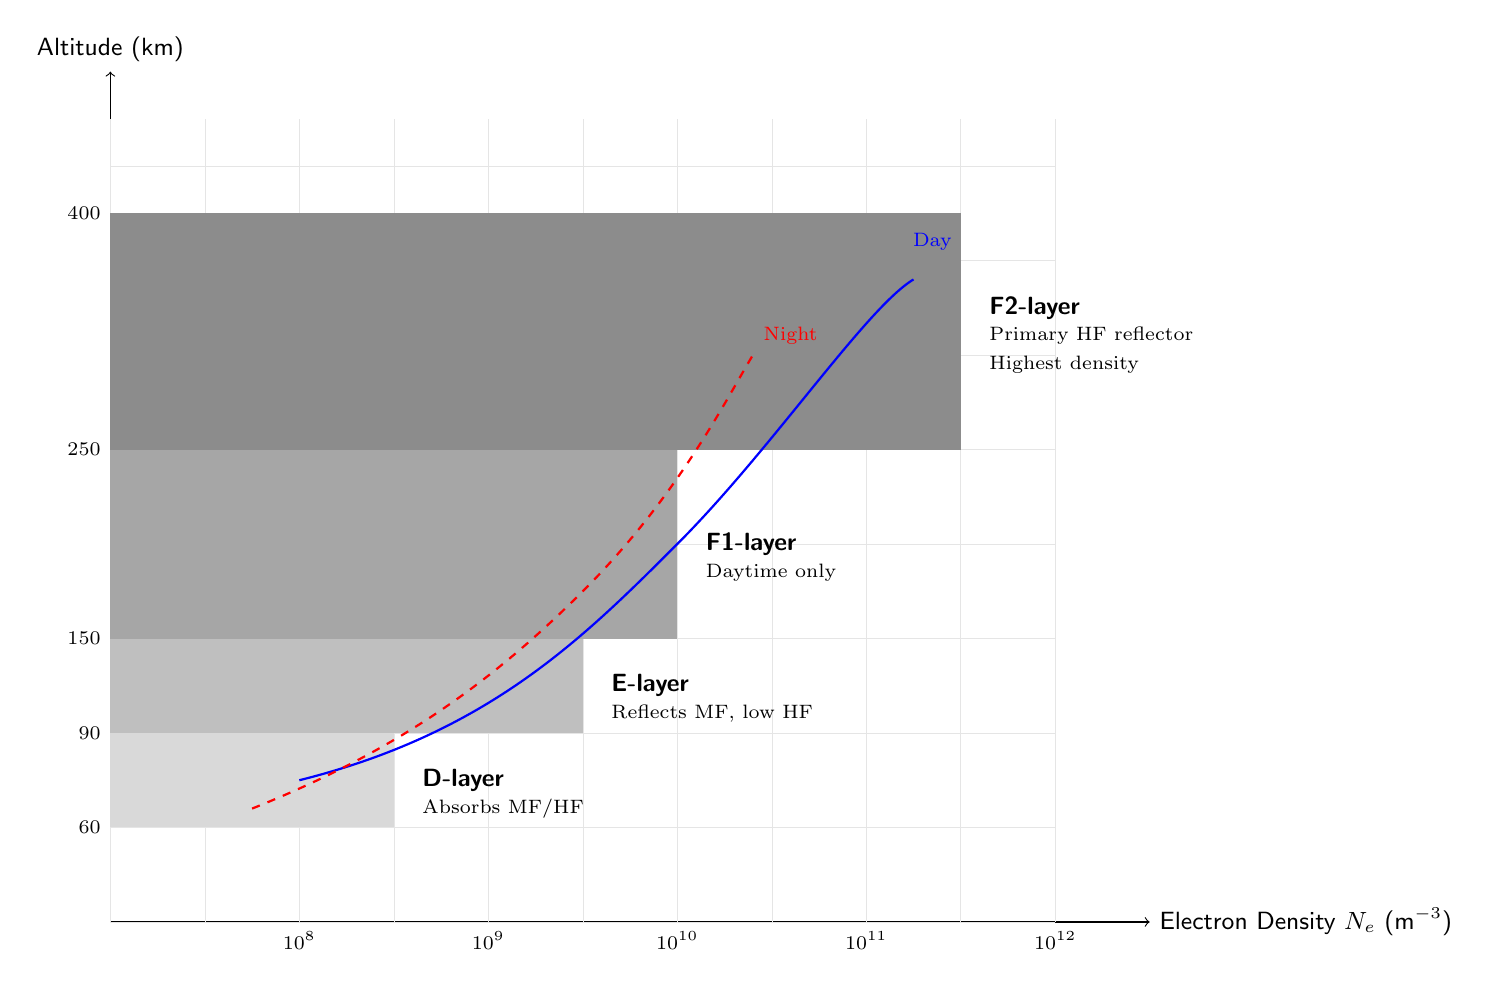
\begin{tikzpicture}[scale=1.2]
% Altitude axis
\draw[->] (0,0) -- (0,9) node[above] {\sffamily\small Altitude (km)};
\draw[->] (0,0) -- (11,0) node[right] {\sffamily\small Electron Density $N_e$ (m$^{-3}$)};

% Grid
\draw[very thin,gray!20] (0,0) grid[step=1] (10,8.5);

% Altitude labels
\node[left,font=\scriptsize] at (0,1) {60};
\node[left,font=\scriptsize] at (0,2) {90};
\node[left,font=\scriptsize] at (0,3) {150};
\node[left,font=\scriptsize] at (0,5) {250};
\node[left,font=\scriptsize] at (0,7.5) {400};

% Electron density labels
\node[below,font=\scriptsize] at (2,0) {10$^8$};
\node[below,font=\scriptsize] at (4,0) {10$^9$};
\node[below,font=\scriptsize] at (6,0) {10$^{10}$};
\node[below,font=\scriptsize] at (8,0) {10$^{11}$};
\node[below,font=\scriptsize] at (10,0) {10$^{12}$};

% D-layer (60-90 km)
\fill[black!15] (0,1) rectangle (3,2);
\node[right,font=\sffamily\small\bfseries] at (3.2,1.5) {D-layer};
\node[right,font=\scriptsize] at (3.2,1.2) {Absorbs MF/HF};

% E-layer (90-150 km)
\fill[black!25] (0,2) rectangle (5,3);
\node[right,font=\sffamily\small\bfseries] at (5.2,2.5) {E-layer};
\node[right,font=\scriptsize] at (5.2,2.2) {Reflects MF, low HF};

% F1-layer (150-250 km) - daytime only
\fill[black!35] (0,3) rectangle (6,5);
\node[right,font=\sffamily\small\bfseries] at (6.2,4) {F1-layer};
\node[right,font=\scriptsize] at (6.2,3.7) {Daytime only};

% F2-layer (250-400 km)
\fill[black!45] (0,5) rectangle (9,7.5);
\node[right,font=\sffamily\small\bfseries] at (9.2,6.5) {F2-layer};
\node[right,font=\scriptsize] at (9.2,6.2) {Primary HF reflector};
\node[right,font=\scriptsize] at (9.2,5.9) {Highest density};

% Day/Night profile curves (schematic)
\draw[thick,blue] (2,1.5) .. controls (4,2) and (5,3) .. (6,4) .. controls (7,5) and (8,6.5) .. (8.5,6.8);
\node[blue,font=\scriptsize] at (8.7,7.2) {Day};

\draw[thick,red,dashed] (1.5,1.2) .. controls (3,1.8) and (4,2.5) .. (5,3.5) .. controls (6,4.5) and (6.5,5.5) .. (6.8,6);
\node[red,font=\scriptsize] at (7.2,6.2) {Night};
\end{tikzpicture}
\end{center}

{\def\LTcaptype{} % do not increment counter
\begin{longtable}[]{@{}
  >{\raggedright\arraybackslash}p{(\linewidth - 6\tabcolsep) * \real{0.1250}}
  >{\raggedright\arraybackslash}p{(\linewidth - 6\tabcolsep) * \real{0.1786}}
  >{\raggedright\arraybackslash}p{(\linewidth - 6\tabcolsep) * \real{0.3929}}
  >{\raggedright\arraybackslash}p{(\linewidth - 6\tabcolsep) * \real{0.3036}}@{}}
\toprule\noalign{}
\begin{minipage}[b]{\linewidth}\raggedright
Layer
\end{minipage} & \begin{minipage}[b]{\linewidth}\raggedright
Altitude
\end{minipage} & \begin{minipage}[b]{\linewidth}\raggedright
Peak Density (\(N_e\))
\end{minipage} & \begin{minipage}[b]{\linewidth}\raggedright
Characteristics
\end{minipage} \\
\midrule\noalign{}
\endhead
\bottomrule\noalign{}
\endlastfoot
\textbf{D} & 60-90 km &
$10^8$--$10^9$ e$^-$/m$^3$
& \textbf{Absorbs MF/HF} (daytime only) \\
\textbf{E} & 90-150 km &
$10^{10}$--$10^{11}$ e$^-$/m$^3$
& Reflects MF, low HF \\
\textbf{F1} & 150-250 km &
$10^{11}$ e$^-$/m$^3$
& Daytime only, merges with F2 at night \\
\textbf{F2} & 250-400 km &
$10^{11}$--$10^{12}$ e$^-$/m$^3$
& \textbf{Primary HF reflector}, highest density \\
\end{longtable}
}

\textbf{Formation mechanism:} Solar UV photons ionize atmospheric molecules:
\begin{equation}
\mathrm{O}_2 + h\nu \rightarrow \mathrm{O}_2^+ + e^-
\end{equation}
where:
\begin{itemize}
\item $h\nu$ = solar UV/X-ray photon energy
\item $\mathrm{O}_2^+$ = ionized oxygen molecule
\item $e^-$ = free electron
\end{itemize}

\textbf{Recombination:} Electrons recombine with ions (faster at lower altitudes due to higher atmospheric density). This creates the altitude-dependent layer structure.

\subsection{Plasma Refractive Index}

The refractive index of ionized plasma determines how radio waves propagate:
\begin{equation}
n = \sqrt{1 - \frac{f_p^2}{f^2}}
\end{equation}
where:
\begin{itemize}
\item $n$ = refractive index (dimensionless)
\item $f_p$ = plasma frequency (Hz)
\item $f$ = signal frequency (Hz)
\end{itemize}

The \textbf{plasma frequency} depends on electron density:
\begin{equation}
f_p = 9\sqrt{N_e} \quad \text{(Hz)}
\end{equation}
where:
\begin{itemize}
\item $N_e$ = electron density (electrons/m$^3$)
\item Factor of 9 comes from fundamental constants: $\sqrt{e^2/(4\pi^2 \epsilon_0 m_e)}$
\end{itemize}

\textbf{Physical interpretation:} Three regimes exist:

\begin{enumerate}
\item \textbf{$f \ll f_p$:} Wave is \textbf{reflected} (refractive index becomes imaginary)---enables HF sky-wave propagation
\item \textbf{$f \approx f_p$:} Wave \textbf{refracts strongly} (bends back toward Earth)---critical frequency behavior
\item \textbf{$f \gg f_p$:} Wave \textbf{penetrates} ionosphere (refractive index $\approx$ 1)---VHF and above pass through
\end{enumerate}

\begin{calloutbox}{Typical Plasma Frequency Values}
\begin{tabular}{@{}ll@{}}
\toprule
Layer & Plasma Frequency \\
\midrule
D-layer & $\sim$1~MHz \\
E-layer & $\sim$3--5~MHz \\
F2-layer (daytime) & $\sim$10--15~MHz \\
F2-layer (nighttime) & $\sim$5--10~MHz \\
\bottomrule
\end{tabular}
\end{calloutbox}

\begin{keyconcept}
\textbf{VHF and above ($>$30~MHz) always penetrate} the ionosphere because $f \gg f_p$ for all layers. This means:
\begin{itemize}
\item No sky-wave propagation above 30~MHz
\item Only line-of-sight (LOS) propagation possible
\item Satellite communications unaffected by ionospheric reflection
\end{itemize}
\end{keyconcept}

\subsection{Critical Frequency and Maximum Usable Frequency}

The \textbf{critical frequency} $f_c$ is the maximum frequency that can be reflected at vertical incidence:
\begin{equation}
f_c = 9\sqrt{N_{e,\text{max}}}
\end{equation}
where:
\begin{itemize}
\item $f_c$ = critical frequency (Hz)
\item $N_{e,\text{max}}$ = peak electron density in layer (electrons/m$^3$)
\end{itemize}

At oblique angles, higher frequencies can be reflected. The \textbf{Maximum Usable Frequency (MUF)} is:
\begin{equation}
\text{MUF} = \frac{f_c}{\sin(\theta)}
\end{equation}
where:
\begin{itemize}
\item MUF = maximum usable frequency (Hz)
\item $\theta$ = elevation angle from horizontal
\end{itemize}

\begin{center}
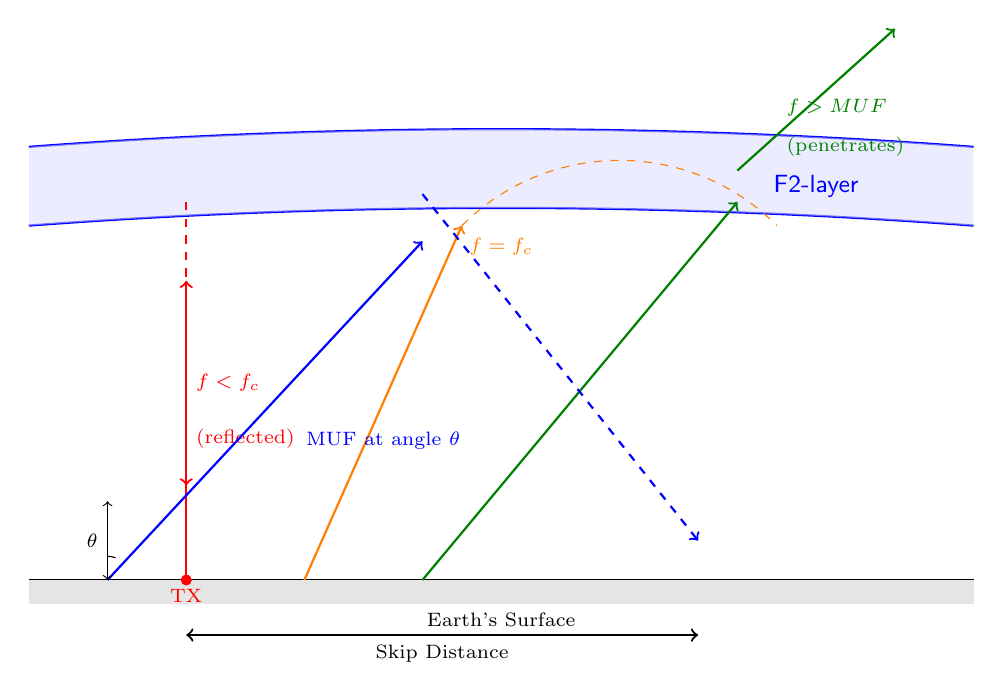
\begin{tikzpicture}[scale=1.0]
% Earth surface
\draw[thick,black] (0,0) -- (12,0);
\fill[black!10] (0,-0.3) rectangle (12,0);
\node[below,font=\scriptsize] at (6,-0.3) {Earth's Surface};

% Ionosphere layer
\draw[thick,blue] (0,4.5) .. controls (4,4.8) and (8,4.8) .. (12,4.5);
\draw[thick,blue] (0,5.5) .. controls (4,5.8) and (8,5.8) .. (12,5.5);
\fill[blue!15,opacity=0.5] (0,4.5) .. controls (4,4.8) and (8,4.8) .. (12,4.5)
  -- (12,5.5) .. controls (8,5.8) and (4,5.8) .. (0,5.5) -- cycle;
\node[blue,font=\sffamily\small] at (10,5) {F2-layer};

% Transmitter
\fill[red] (2,0) circle (2pt);
\node[below,red,font=\scriptsize] at (2,0) {TX};

% Ray 1: Low frequency (reflected, vertical)
\draw[->,thick,red] (2,0) -- (2,3.8);
\draw[->,thick,red,dashed] (2,4.8) -- (2,1.2);
\node[right,red,font=\scriptsize] at (2,2.5) {$f < f_c$};
\node[right,red,font=\scriptsize] at (2,1.8) {(reflected)};

% Ray 2: Critical frequency (grazes ionosphere)
\draw[->,thick,orange] (3.5,0) -- (5.5,4.5);
\draw[orange,dashed] (5.5,4.5) arc (135:45:2.83);
\node[above,orange,font=\scriptsize] at (6,4) {$f = f_c$};

% Ray 3: Higher frequency (penetrates)
\draw[->,thick,green!50!black] (5,0) -- (9,4.8);
\draw[->,thick,green!50!black] (9,5.2) -- (11,7);
\node[right,green!50!black,font=\scriptsize] at (9.5,6) {$f > \text{MUF}$};
\node[right,green!50!black,font=\scriptsize] at (9.5,5.5) {(penetrates)};

% Ray 4: Oblique MUF (just reflected)
\draw[->,thick,blue] (1,0) -- (5,4.3);
\draw[->,thick,blue,dashed] (5,4.9) -- (8.5,0.5);
\node[below,blue,font=\scriptsize] at (4.5,2) {MUF at angle $\theta$};

% Angle annotation
\draw[<->,thin] (1,0) -- (1,1) node[midway,left,font=\scriptsize] {$\theta$};
\draw (1,0.3) arc (90:70:0.3);

% Skip distance
\draw[<->,thick] (2,-0.7) -- (8.5,-0.7) node[midway,below,font=\scriptsize] {Skip Distance};
\end{tikzpicture}
\end{center}

\textbf{Example calculation:}

If $f_c = 10$~MHz and a wave is launched at $\theta = 10°$ elevation:
\begin{equation}
\text{MUF} = \frac{10\text{~MHz}}{\sin(10°)} = \frac{10}{0.174} = 57.5\text{~MHz}
\end{equation}

In practice, MUF is limited to $\sim$30~MHz by D-layer absorption and other factors.

\subsection{D-Layer Absorption}

The D-layer causes signal attenuation through collisional damping:
\begin{equation}
A = K \cdot \frac{N_e \cdot \nu}{f^2} \quad \text{(dB)}
\end{equation}
where:
\begin{itemize}
\item $A$ = absorption (dB)
\item $K$ = constant depending on path geometry
\item $N_e$ = electron density (electrons/m$^3$)
\item $\nu$ = collision frequency ($\sim$10$^6$~Hz in D-layer)
\item $f$ = signal frequency (Hz)
\end{itemize}

\begin{keyconcept}
\textbf{Absorption is inversely proportional to frequency squared:} $A \propto 1/f^2$

This means lower frequencies experience much more absorption. A 3~MHz signal absorbs \textbf{100 times more} than a 30~MHz signal in the same ionospheric path.
\end{keyconcept}

\textbf{Day/Night variation:}
\begin{itemize}
\item \textbf{Daytime:} D-layer strongly absorbs MF/LF (1--5~MHz), severe attenuation
\item \textbf{Nighttime:} D-layer disappears $\rightarrow$ lower frequencies propagate via sky-wave (enables AM broadcast reception)
\end{itemize}

\begin{calloutbox}{Typical HF Absorption (Daytime)}
\begin{tabular}{@{}ll@{}}
\toprule
Frequency & Typical Absorption \\
\midrule
3~MHz & 10--20~dB \\
7~MHz & 3--6~dB \\
14~MHz & 1--2~dB \\
28~MHz & $<$1~dB \\
\bottomrule
\end{tabular}
\end{calloutbox}

\subsection{Faraday Rotation}

The ionosphere is embedded in Earth's magnetic field, causing \textbf{polarization rotation} as electromagnetic waves propagate:
\begin{equation}
\Omega = \frac{2.36 \times 10^4}{f^2} \int N_e B_\parallel \, dl \quad \text{(radians)}
\end{equation}
where:
\begin{itemize}
\item $\Omega$ = total polarization rotation angle (radians)
\item $f$ = signal frequency (Hz)
\item $N_e$ = electron density along path (electrons/m$^3$)
\item $B_\parallel$ = magnetic field component parallel to propagation (Tesla)
\item $dl$ = differential path element (m)
\end{itemize}

\textbf{Physical mechanism:} Left and right circularly polarized components travel at different velocities in magnetized plasma, causing the linear polarization vector to rotate.

\begin{warningbox}
\textbf{Linear polarized signals experience severe losses} if the receive antenna is cross-polarized to the rotated signal. Faraday rotation can cause $>$20~dB loss in worst-case misalignment.

\textbf{Mitigation:} Use circular polarization (RHCP/LHCP), which is immune to Faraday rotation. This is why GPS and satellite communications systems use circular polarization.
\end{warningbox}

\textbf{Example:} GPS L1 (1575~MHz) experiences $\sim$10--50$°$ rotation depending on:
\begin{itemize}
\item Solar activity (higher during solar maximum)
\item Latitude (stronger near magnetic poles)
\item Time of day (peak at local noon)
\end{itemize}



\subsection{Ionospheric Delay}

Radio signals travel \textbf{slower through ionized plasma} than through free space, causing group delay:
\begin{equation}
\Delta t = \frac{40.3}{c f^2} \int N_e \, dl \quad \text{(seconds)}
\end{equation}
where:
\begin{itemize}
\item $\Delta t$ = group delay (seconds)
\item $c$ = speed of light (3$\times$10$^8$~m/s)
\item $f$ = signal frequency (Hz)
\item $N_e$ = electron density (electrons/m$^3$)
\item $dl$ = path element (m)
\end{itemize}

This delay is quantified using \textbf{Total Electron Content (TEC)}:
\begin{equation}
\text{TEC} = \int N_e \, dl \quad \text{(electrons/m$^2$)}
\end{equation}

The ranging error caused by ionospheric delay is:
\begin{equation}
\Delta R = c \cdot \Delta t = \frac{40.3 \cdot \text{TEC}}{f^2} \quad \text{(meters)}
\end{equation}
where:
\begin{itemize}
\item $\Delta R$ = ranging error (m)
\item TEC = total electron content (electrons/m$^2$)
\item $f$ = frequency (Hz)
\end{itemize}

\begin{calloutbox}{Typical TEC Values}
\begin{tabular}{@{}ll@{}}
\toprule
Condition & TEC (electrons/m$^2$) \\
\midrule
Nighttime & 10$^{16}$ \\
Daytime (mid-latitude) & 10$^{17}$ \\
Solar maximum (equatorial) & 10$^{18}$ \\
\bottomrule
\end{tabular}
\end{calloutbox}

\textbf{GPS error example:} At L1 frequency (1575~MHz) with TEC $= 5 \times 10^{17}$:
\begin{equation}
\Delta R = \frac{40.3 \times 5 \times 10^{17}}{(1.575 \times 10^9)^2} \approx 8.1\text{~m}
\end{equation}

\textbf{Dual-frequency correction:} Measure delay at two frequencies (L1 and L5) to compute TEC and remove error:
\begin{equation}
\text{TEC} = \frac{f_1^2 f_2^2}{40.3(f_1^2 - f_2^2)}(\Delta t_1 - \Delta t_2)
\end{equation}

\section{Tropospheric Effects}

The \textbf{troposphere} is the lower atmosphere (0--15~km altitude) where weather occurs. It affects RF propagation through three primary mechanisms:

\begin{enumerate}
\item \textbf{Refraction:} Bending of rays due to density gradients
\item \textbf{Absorption:} Molecular resonances (O$_2$, H$_2$O) attenuate signals
\item \textbf{Scattering:} Rain, fog, and turbulence scatter energy
\end{enumerate}

\subsection{Atmospheric Refraction}

The tropospheric refractive index varies with altitude due to changes in temperature, pressure, and humidity:
\begin{equation}
n = 1 + N \times 10^{-6}
\end{equation}
where:
\begin{itemize}
\item $n$ = refractive index (dimensionless)
\item $N$ = refractivity (dimensionless)
\end{itemize}

The \textbf{refractivity} is given by:
\begin{equation}
N = 77.6 \frac{P}{T} + 3.73 \times 10^5 \frac{e}{T^2}
\end{equation}
where:
\begin{itemize}
\item $P$ = atmospheric pressure (hPa or mbar)
\item $T$ = temperature (K)
\item $e$ = water vapor partial pressure (hPa)
\end{itemize}

The first term represents the \textbf{dry atmosphere} contribution, while the second term accounts for \textbf{water vapor} (more significant in humid conditions).

\begin{calloutbox}{Typical Refractivity Values}
\begin{tabular}{@{}ll@{}}
\toprule
Location & Refractivity $N$ \\
\midrule
Sea level (standard) & 300--400 $\rightarrow$ $n \approx 1.0003$ \\
10~km altitude & $\sim$100 $\rightarrow$ $n \approx 1.0001$ \\
Dry desert & 250--300 \\
Humid tropics & 350--400 \\
\bottomrule
\end{tabular}
\end{calloutbox}

\subsection{Ray Bending and Extended Horizon}

The vertical gradient in refractivity causes radio rays to bend downward, following Earth's curvature more closely than optical rays.

\textbf{Standard atmosphere gradient:}
\begin{equation}
\frac{dN}{dh} \approx -40 \text{~N-units/km}
\end{equation}
where $h$ is altitude (km).

This bending \textbf{extends the radio horizon} beyond the geometric horizon. The effect is modeled using the \textbf{4/3 Earth radius model}:
\begin{equation}
d_{\text{radio}} = 1.33 \times d_{\text{geometric}}
\end{equation}
where:
\begin{itemize}
\item $d_{\text{radio}}$ = radio line-of-sight distance (km)
\item $d_{\text{geometric}}$ = geometric horizon distance (km)
\end{itemize}

The geometric horizon distance for an antenna at height $h$ (meters) is:
\begin{equation}
d_{\text{geometric}} = 3.57\sqrt{h} \quad \text{(km)}
\end{equation}

Therefore, the radio horizon is:
\begin{equation}
d_{\text{radio}} = 4.12\sqrt{h} \quad \text{(km)}
\end{equation}

\textbf{Example:} For a 30~m antenna height:
\begin{equation}
d_{\text{radio}} = 4.12\sqrt{30} = 22.6\text{~km}
\end{equation}

This is approximately 33\% farther than the geometric horizon (17~km).

\subsection{Tropospheric Ducting}

\textbf{Temperature inversion} (warm air over cool air) creates a refractive layer that traps radio waves, enabling \textbf{super-refraction}.

\begin{center}
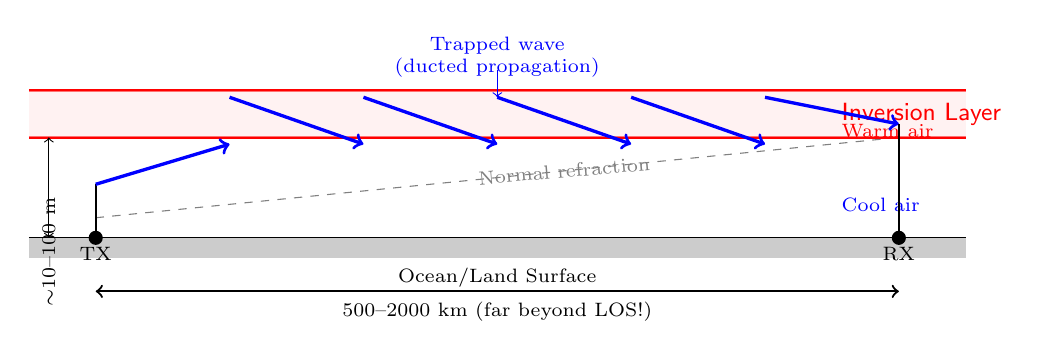
\begin{tikzpicture}[scale=0.85]
% Earth surface
\draw[thick] (0,0) -- (14,0);
\fill[black!20] (0,-0.3) rectangle (14,0);
\node[below,font=\scriptsize] at (7,-0.3) {Ocean/Land Surface};

% Normal atmosphere (dashed line showing normal propagation)
\draw[thin,gray,dashed] (1,0.3) -- (13,1.5);
\node[gray,font=\scriptsize,rotate=5] at (8,1) {Normal refraction};

% Temperature inversion layer
\draw[thick,red] (0,1.5) -- (14,1.5);
\draw[thick,red] (0,2.2) -- (14,2.2);
\fill[red!10,opacity=0.5] (0,1.5) rectangle (14,2.2);
\node[red,font=\sffamily\small,right] at (12,1.85) {Inversion Layer};
\node[red,font=\scriptsize,right] at (12,1.6) {Warm air};

% Cool air below
\node[blue,font=\scriptsize,right] at (12,0.5) {Cool air};

% Transmitter
\fill[black] (1,0) circle (3pt);
\node[below,font=\scriptsize] at (1,0) {TX};
\draw[thick] (1,0) -- (1,0.8);

% Ducted ray (bounces within duct)
\draw[->,thick,blue,line width=1.2pt] (1,0.8) -- (3,1.4);
\draw[->,thick,blue,line width=1.2pt] (3,2.1) -- (5,1.4);
\draw[->,thick,blue,line width=1.2pt] (5,2.1) -- (7,1.4);
\draw[->,thick,blue,line width=1.2pt] (7,2.1) -- (9,1.4);
\draw[->,thick,blue,line width=1.2pt] (9,2.1) -- (11,1.4);
\draw[->,thick,blue,line width=1.2pt] (11,2.1) -- (13,1.7);

% Receiver
\fill[black] (13,0) circle (3pt);
\node[below,font=\scriptsize] at (13,0) {RX};
\draw[thick] (13,0) -- (13,1.7);

% Distance annotation
\draw[<->,thick] (1,-0.8) -- (13,-0.8) node[midway,below,font=\scriptsize] {500--2000 km (far beyond LOS!)};

% Height annotation
\draw[<->,thin] (0.3,0) -- (0.3,1.5) node[midway,left,font=\scriptsize,rotate=90] {$\sim$10--100 m};

% Ray path annotation
\node[blue,font=\scriptsize,align=center] at (7,2.7) {Trapped wave\\(ducted propagation)};
\draw[->,blue] (7,2.5) -- (7,2.1);
\end{tikzpicture}
\end{center}

\textbf{Mechanism:} The refractive index gradient is stronger than normal, causing radio waves to bend sharply downward and become \textbf{trapped in a waveguide} between the surface and inversion layer.

\textbf{Conditions favoring ducting:}
\begin{itemize}
\item \textbf{Coastal regions:} Cool ocean air beneath warm land air
\item \textbf{High-pressure systems:} Stable, clear weather with subsidence
\item \textbf{Nighttime:} Radiative cooling creates surface inversion
\end{itemize}

\textbf{Effects:}
\begin{itemize}
\item \textbf{VHF/UHF signals propagate 500--2000~km} (far beyond normal line-of-sight)
\item FM/TV interference from distant stations
\item Cellular network interference (distant cells suddenly become visible)
\item Opportunistic long-range VHF communications
\end{itemize}

\textbf{Duct characteristics:}
\begin{itemize}
\item Height: Typically 10--100~m (depends on inversion strength)
\item Duration: Hours to days
\item Frequency: Most effective for VHF/UHF (30--3000~MHz)
\end{itemize}



\subsection{Atmospheric Windows}

Certain frequency ranges experience low atmospheric absorption, creating \textbf{atmospheric windows} suitable for wireless communications.

\begin{center}
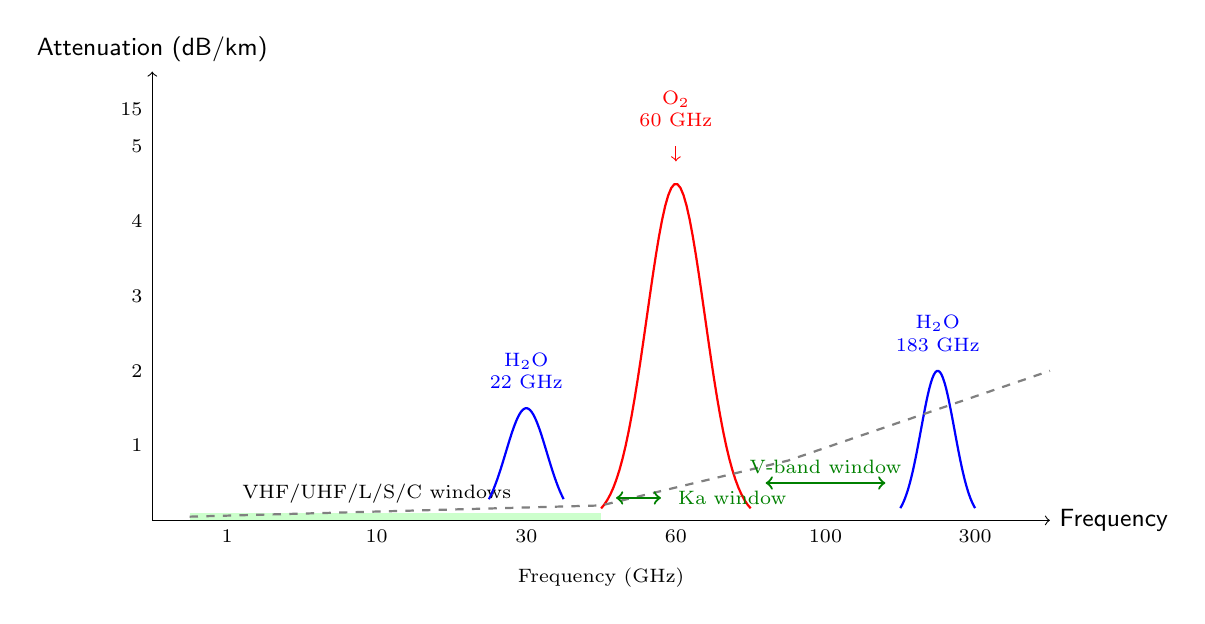
\begin{tikzpicture}[scale=0.95]
% Axes
\draw[->] (0,0) -- (12,0) node[right,font=\sffamily\small] {Frequency};
\draw[->] (0,0) -- (0,6) node[above,font=\sffamily\small] {Attenuation (dB/km)};

% Frequency labels (logarithmic spacing)
\node[below,font=\scriptsize] at (1,0) {1};
\node[below,font=\scriptsize] at (3,0) {10};
\node[below,font=\scriptsize] at (5,0) {30};
\node[below,font=\scriptsize] at (7,0) {60};
\node[below,font=\scriptsize] at (9,0) {100};
\node[below,font=\scriptsize] at (11,0) {300};
\node[below,font=\scriptsize] at (6,-0.5) {Frequency (GHz)};

% Attenuation labels
\foreach \y in {1,2,3,4,5}
  \node[left,font=\scriptsize] at (0,\y) {\y};
\node[left,font=\scriptsize] at (0,5.5) {15};

% Low absorption regions (windows)
\fill[green!20] (0.5,0) rectangle (6,0.1);
\node[above,font=\scriptsize] at (3,0.1) {VHF/UHF/L/S/C windows};

% O2 absorption peak at 60 GHz
\draw[thick,red,domain=6:8,samples=50] plot (\x, {4.5*exp(-(\x-7)^2/0.3)});
\node[red,font=\scriptsize,align=center] at (7,5.5) {O$_2$\\60 GHz};
\draw[->,red] (7,5) -- (7,4.8);

% H2O absorption at 22 GHz
\draw[thick,blue,domain=4.5:5.5,samples=50] plot (\x, {1.5*exp(-(\x-5)^2/0.15)});
\node[blue,font=\scriptsize,align=center] at (5,2) {H$_2$O\\22 GHz};

% H2O absorption at 183 GHz (schematic, off-scale)
\draw[thick,blue,domain=10:11,samples=50] plot (\x, {2*exp(-(\x-10.5)^2/0.1)});
\node[blue,font=\scriptsize,align=center] at (10.5,2.5) {H$_2$O\\183 GHz};

% General trend line (increasing with frequency)
\draw[thick,gray,dashed] (0.5,0.05) -- (6,0.2) -- (8.5,0.8) -- (12,2);

% Window annotations
\draw[<->,thick,green!50!black] (6.2,0.3) -- (6.8,0.3);
\node[right,green!50!black,font=\scriptsize] at (6.9,0.3) {Ka window};

\draw[<->,thick,green!50!black] (8.2,0.5) -- (9.8,0.5);
\node[above,green!50!black,font=\scriptsize] at (9,0.5) {V-band window};
\end{tikzpicture}
\end{center}

\begin{calloutbox}{Atmospheric Windows and Applications}
\begin{tabular}{@{}lll@{}}
\toprule
Band & Frequency & Typical Use \\
\midrule
VHF/UHF & 30--3000~MHz & Broadcast, cellular \\
L/S-band & 1--4~GHz & GPS, mobile satellite \\
C-band & 4--8~GHz & Satellite (rain-robust) \\
X/Ku-band & 8--18~GHz & Satellite, radar \\
Ka-band & 26.5--40~GHz & High-rate satellite \\
V/W-band & 40--100~GHz & Point-to-point links \\
\bottomrule
\end{tabular}
\end{calloutbox}

\begin{warningbox}
\textbf{Avoid these absorption peaks:}
\begin{itemize}
\item \textbf{22~GHz:} Water vapor (H$_2$O) resonance
\item \textbf{60~GHz:} Oxygen (O$_2$) resonance---15~dB/km attenuation!
\item \textbf{183~GHz:} Strong water vapor resonance
\end{itemize}

The 60~GHz oxygen peak is exploited for \textbf{secure short-range communications} where signals naturally attenuate over distance.
\end{warningbox}



\section{Worked Example: Satellite Link with Atmospheric Effects}

\textbf{Scenario:} Design a Ku-band satellite downlink from geostationary orbit

\subsection*{Given Parameters}

\begin{tabular}{@{}ll@{}}
Satellite altitude & 36,000~km (GEO) \\
Frequency & 12~GHz (Ku-band) \\
Elevation angle & 30$°$ \\
TX power & $P_t = 50$~W (47~dBm) \\
TX antenna gain & $G_t = 30$~dBi \\
RX antenna gain & $G_r = 40$~dBi (1~m dish) \\
System noise temp & $T_s = 150$~K \\
Bandwidth & $B = 36$~MHz \\
Required BER & $10^{-6}$ (QPSK) \\
Location & Temperate climate \\
\end{tabular}

\subsection*{Step 1: Free-Space Path Loss}

The free-space path loss is:
\begin{equation}
\text{FSPL} = 20\log_{10}(d) + 20\log_{10}(f) + 92.45 \quad \text{(dB)}
\end{equation}
where $d$ is in km and $f$ is in MHz.

\begin{equation}
\text{FSPL} = 20\log_{10}(36{,}000) + 20\log_{10}(12{,}000) + 92.45 = 205.5\text{~dB}
\end{equation}

\subsection*{Step 2: Clear-Air Atmospheric Absorption}

At 12~GHz, clear-air atmospheric absorption (zenith):
\begin{equation}
L_{\text{atm,zenith}} \approx 0.3\text{~dB}
\end{equation}

For elevation angle $\theta = 30°$, the slant path is longer:
\begin{equation}
L_{\text{atm}} = \frac{L_{\text{atm,zenith}}}{\sin(\theta)} = \frac{0.3}{\sin(30°)} = 0.6\text{~dB}
\end{equation}

\subsection*{Step 3: Rain Fade Margin}

For 99.9\% availability in temperate climate at Ku-band:
\begin{equation}
L_{\text{rain}} = 3\text{~dB}
\end{equation}

\subsection*{Step 4: Scintillation Margin}

Tropospheric scintillation at 12~GHz, 30$°$ elevation:
\begin{equation}
L_{\text{scint}} = 1\text{~dB}
\end{equation}

\subsection*{Step 5: Total Path Loss}

The total path loss including all atmospheric effects:
\begin{equation}
L_{\text{total}} = \text{FSPL} + L_{\text{atm}} + L_{\text{rain}} + L_{\text{scint}}
\end{equation}
\begin{equation}
L_{\text{total}} = 205.5 + 0.6 + 3 + 1 = 210.1\text{~dB}
\end{equation}

\subsection*{Step 6: Received Signal Power}

The received power is:
\begin{equation}
P_r = P_t + G_t + G_r - L_{\text{total}}
\end{equation}
\begin{equation}
P_r = 47 + 30 + 40 - 210.1 = -93.1\text{~dBm}
\end{equation}

\subsection*{Step 7: Noise Power}

The noise power is:
\begin{equation}
N = 10\log_{10}(kT_sB) = 10\log_{10}(1.38 \times 10^{-23} \times 150 \times 36 \times 10^6)
\end{equation}
\begin{equation}
N = -113.4\text{~dBm}
\end{equation}

\subsection*{Step 8: Carrier-to-Noise Ratio}

\begin{equation}
\frac{C}{N} = P_r - N = -93.1 - (-113.4) = 20.3\text{~dB}
\end{equation}

\subsection*{Step 9: Required C/N for BER $= 10^{-6}$}

For QPSK with BER $= 10^{-6}$:
\begin{equation}
\left(\frac{E_b}{N_0}\right)_{\text{req}} = 10.5\text{~dB}
\end{equation}

For data rate $R_b = 72$~Mbps (2 bits/symbol, 36~MHz bandwidth):
\begin{equation}
\left(\frac{C}{N}\right)_{\text{req}} = \left(\frac{E_b}{N_0}\right)_{\text{req}} + 10\log_{10}\left(\frac{R_b}{B}\right) = 10.5 + 3 = 13.5\text{~dB}
\end{equation}

\subsection*{Step 10: Link Margin}

\begin{equation}
\text{Margin} = \frac{C}{N} - \left(\frac{C}{N}\right)_{\text{req}} = 20.3 - 13.5 = 6.8\text{~dB}
\end{equation}

\begin{calloutbox}[colback=black!8!white,colframe=black]{Link Budget Summary}
\textbf{Result: Link closes with 6.8~dB margin}

This margin provides headroom for:
\begin{itemize}
\item Implementation losses (2--3~dB)
\item Pointing errors (1--2~dB)
\item Unexpected fading events
\item Component aging
\end{itemize}

\textbf{Conclusion:} The link is viable for reliable 72~Mbps QPSK transmission with atmospheric effects accounted for. The atmospheric contributions total 4.6~dB (0.6 + 3 + 1), representing \textbf{2.2\% of the total path loss}.
\end{calloutbox}



\section{Applications}

\subsection{HF Long-Distance Communications}

\textbf{System:} Shortwave radio, amateur radio, military HF
\begin{itemize}
\item \textbf{Frequency:} 3--30~MHz
\item \textbf{Ionospheric layer:} F2-layer reflection
\item \textbf{Range:} Global (multi-hop propagation)
\item \textbf{Advantage:} No infrastructure required (over-the-horizon)
\item \textbf{Challenge:} Variable propagation with solar activity
\end{itemize}

\subsection{GPS and GNSS Navigation}

\textbf{System:} GPS, Galileo, GLONASS
\begin{itemize}
\item \textbf{Frequency:} L-band (1--2~GHz)
\item \textbf{Effect:} Ionospheric delay causes ranging errors
\item \textbf{Mitigation:} Dual-frequency correction (L1 + L5)
\item \textbf{Typical error:} 10--30~m (single frequency), $<$1~m (dual frequency)
\item \textbf{Key parameter:} Total Electron Content (TEC) monitoring
\end{itemize}

\subsection{Satellite Communications}

\textbf{System:} Ku/Ka-band satellite links
\begin{itemize}
\item \textbf{Frequency:} 12--18~GHz (Ku), 26--40~GHz (Ka)
\item \textbf{Primary effect:} Rain fade, atmospheric absorption
\item \textbf{Design consideration:} Link margin for 99.9\% availability
\item \textbf{Tropospheric loss:} 0.5--1~dB (clear air), 3--13~dB (rain)
\item \textbf{Trade-off:} Higher frequency = smaller antennas but worse weather sensitivity
\end{itemize}

\subsection{VHF/UHF Terrestrial Broadcasting}

\textbf{System:} FM radio, TV broadcasting, cellular networks
\begin{itemize}
\item \textbf{Frequency:} 30--3000~MHz
\item \textbf{Normal propagation:} Line-of-sight (extended by refraction)
\item \textbf{Ducting events:} Occasional long-range propagation (500--2000~km)
\item \textbf{Impact:} Interference from distant stations during atmospheric anomalies
\end{itemize}

\section{Summary}

\begin{center}
\begin{tabular}{@{}lll@{}}
\toprule
\textbf{Frequency Band} & \textbf{Dominant Effect} & \textbf{Key Impact} \\
\midrule
HF (3--30~MHz) & Ionospheric refraction & Sky-wave propagation \\
VHF (30--300~MHz) & Tropospheric refraction & Extended horizon, ducting \\
UHF/L-band (0.3--4~GHz) & Ionospheric delay & GPS ranging errors \\
C-band (4--8~GHz) & Minimal atmospheric & Rain fade (manageable) \\
Ku-band (12--18~GHz) & Rain fade & Moderate weather impact \\
Ka-band (26--40~GHz) & Rain + absorption & Severe weather sensitivity \\
V-band (40--75~GHz) & O$_2$ absorption & 60~GHz peak (15~dB/km) \\
\bottomrule
\end{tabular}
\end{center}

\textbf{Key design principles:}
\begin{itemize}
\item \textbf{Below 30~MHz:} Exploit ionospheric refraction for long-distance propagation
\item \textbf{1--4~GHz:} Account for ionospheric delay in precision ranging (GPS)
\item \textbf{4--18~GHz:} Balance between antenna size and rain fade (satellite communications)
\item \textbf{Above 20~GHz:} Significant rain and atmospheric absorption (requires large margins)
\end{itemize}

\textbf{Atmospheric effects summary:}
\begin{itemize}
\item \textbf{Ionosphere enables} HF long-distance propagation but \textbf{disrupts} GPS/GNSS timing
\item \textbf{Troposphere limits} high-frequency satellite links through absorption and rain fade
\item \textbf{Frequency selection} must balance propagation characteristics with atmospheric constraints
\end{itemize}

\section{Further Reading}

\begin{itemize}
\item \textbf{Chapter~\ref{ch:propagation}:} Propagation Modes---ground wave, sky wave, and line-of-sight mechanisms
\item \textbf{Chapter~\ref{ch:weather}:} Weather Effects---detailed rain fade and fog attenuation models
\item \textbf{Chapter~\ref{ch:fspl}:} Free-Space Path Loss---baseline propagation model before atmospheric effects
\item \textbf{Chapter~\ref{ch:linkbudget}:} Complete Link Budget Analysis---incorporating atmospheric losses into system design
\item \textbf{Chapter~\ref{ch:spectrum}:} Electromagnetic Spectrum---frequency allocation and atmospheric windows
\end{itemize}
